\chapter{Special functions and properties}
This appendix covers the basics of some of the special functions that arise when discussing the properties of some operators in quantum mechanics and formulae used.
\section{Legendre polynomials and spherical Bessel functions}\label{app:Bessel}
\begin{equation}
	Y_{\ell}^m(\theta,\phi) = \frac{(-1)^{{\ell}l+m}}{(2\ell)!!}\bigg[ \frac{(2\ell+1)(\ell-m)}{4\pi(\ell+m)!}\bigg](\sin\theta)^m\frac{\text{d}^{\ell+m}}{(d\cos\theta)^{\ell+m}}[(\sin\theta)^{2\ell}]\exp{i m\phi},
\end{equation}
which satisfy
\begin{equation}
	Y_\ell^{*m}=(-1)^m Y_{l}^{-m}.
\end{equation}
The spherical harmonics are connected to the Legendre polynomials
\begin{equation}
	P_\ell(\cos\theta) = \bigg[ \frac{4\pi}{2\ell+1} \bigg]^{1/2}Y_{l}^0(\theta).
\end{equation}
Another important feature of spherical harmonics is that they form a complete set of functions over the unit sphere. Furthermore, they form an orthonormal set
\begin{equation}\label{orthset}
	\int \text{d}\Omega \, Y_\ell^{*m} Y_{l'}^{m'} = \delta_{mm'}\delta_{ll'}.
\end{equation}
Also, there exists an addition theorem for spherical harmonics
\begin{equation}\label{addition}
	\sum_{m=-\ell} Y_\ell^{*m}(\theta,\phi)Y_\ell^{m}(\theta'.\phi') = \bigg( \frac{2\ell+1}{4\pi}\bigg)^{1/2}Y_\ell^0(\alpha).
\end{equation}
The wave function of a plane wave with wave number $k$ propagating along the $z$ axis can be described by
\begin{align} \label{planewave}
	\text{e}^{ikz}  &= \text{e}^{ikr \cos(\theta)}  \\
	&= \sum_{\ell=0}^\infty A_\ell(r)Y_{\ell,0}(\theta),
\end{align}
where
\begin{equation} \label{besselcoef}
	A_\ell(r) = \int \text{d}\Omega \, Y_{\ell,0}^*(\theta)\text{e}^{ikr\cos(\theta)}  = i^\ell\sqrt{4\pi(2\ell+1)}j_\ell(kr),
\end{equation}
where the last equality shows the coefficient $A_\ell(r)$ can be expressed in terms of a spherical Bessel function $j_\ell(kr)$. Using the addition theorem equation \eqref{planewave} yields the decomposition of a plane wave into spherical Bessel functions
\begin{equation} \label{sphericalbesseldecomp}
	\text{e}^{i\vec{k}\cdot\vec{r}} = 4\pi \sum_{\ell,m}i^\ell j_\ell(kr)Y_\ell^{m*}(\theta,\phi)Y_\ell^{m}(\theta,\phi)
\end{equation}
\section{Hankel transform}
\section{Coulomb wave functions}\label{sec:Coulomb}
The Coulomb wave equation for a charged particle with arbitrary angular momentum and charge is given by 
\begin{equation} \label{Coulomb1}
	\nabla^2\psi +\left( k^2-\frac{2\mu}{\hbar^2}V(r)\right)\psi = 0,
\end{equation}
where $\mu$ is the reduced mass of the system. The radial wave function $u(r)$ satisfied the following differential equation
\begin{equation} \label{Coulomb2}
	\frac{\text{d}^2 u_\ell}{\text{d}r^2}+\left( k^2-\frac{\ell(\ell+1)}{r^2}-\frac{2\mu}{\hbar^2}\frac{Ze^2}{r}\right)u_\ell=0,
\end{equation}
where $Z$ is the product of the charges. Two independent solutions can be found to equation \eqref{Coulomb2} -- these are called the regular and irregular Coulomb wave functions denoted $F_\ell(r)$ and $G_\ell(r)$ respectively. The regular Coulomb wave function $F_\ell(r)$ is a real function that vanishes at $r=0$ and the behaviour of the function is described using a parameter $\eta$ which describes how strongly the Coulomb interaction is
\begin{equation} \label{etafactor}
	\eta = \frac{Zmc\alpha }{\hbar k},
\end{equation}
where $m$ is the mass of the particle, $k$ is the wave number and $\alpha$ is the fine structure constant. The solution to is given by
\begin{equation} \label{solCoul}
	F_\ell(\eta,kr) = C_\ell (\eta) (kr)^{\ell+1}\text{e}^{-ikr}  {}_1 F_1(\ell+1-i\eta,2\ell+2,2ikr),
\end{equation}
where ${}_1F_1(kr)$ is a confluent hypergeometric function and $C_\ell(\eta)$ is a normalization constant given by 
\begin{equation} \label{normalization}
	C_\ell(\eta) = \frac{2^\ell \text{e}^{-\pi\eta/2}\abs{\Gamma(\ell+1+i\eta)}}{(2\ell+1)!},
\end{equation}
where $\Gamma$ is the gamma function. For numerical purposes, it is useful to use the integral representation of equation \eqref{solCoul} \cite[eq. 33.7.1]{NIST} 
\begin{equation} \label{integralrep}
	F_\ell(\eta,\rho) = \frac{\rho^{\ell+1}2^\ell e^{i\rho-(\pi\eta/2)}}{|\Gamma(\ell+1+i\eta)|} \int_0^1 e^{-2i\rho t}t^{\ell+i\eta}(1-t)^{\ell-i\eta} \, \text{d}t.
\end{equation}
For particles without charge, we can ignore the Coulomb interaction in equation \eqref{Coulomb2} and the solution becomes \cite{Blatt}
\begin{equation} \label{solcharge}
	F_\ell(kr) = \left( \frac{\pi kr}{2} \right)^{1/2} J_{\ell+1/2}(kr), \quad \text{particles without charge}
\end{equation}
where $J_{\ell+1/2}$ is a Bessel function. Equation \eqref{solcharge} is nothing but a spherical Bessel function. This means in the limit where the particles become chargeless the solution must reduce to a plane wave solution. 

\chapter{Three component wavefunction}\label{ThreeComponentWavefunction}
Strictly speaking, the nuclear model should be consistent with other results from nuclear physics. In particular, the mass difference between the charged pion and the neutral pion. A priori we do not know the impact on the wave function of the nucleon-pion system and in this appendix, we wish to estimate how the wave function changes when we take the different properties of the pion into account. Starting from \eqref{bareproton} and \eqref{pionnuc}
\begin{equation}\label{pnpipi}
	\psi_p = p\uparrow\frac{1}{\sqrt{V}}, \quad \psi_{N\pi^0}=(\vec{\tau\cdot\vec{\pi}})(\vec{\sigma}\cdot\vec{r})\phi_0(r) p\uparrow\frac{1}{\sqrt{V}}, \quad \psi_{N\pi^+}=(\vec{\tau\cdot\vec{\pi}})(\vec{\sigma}\cdot\vec{r})\phi_+(r) p\uparrow\frac{1}{\sqrt{V}},
\end{equation}
and these will act as the state vector in our system. Constructing a similar Hamiltonian for the three-component wave function yields
\begin{equation}
	\mqty[K_{\vec{p}} & W^\dagger & W^\dagger \\ W & K_{\vec{p}}+K_0+m_{\pi^0} & 0 \\ W & 0 & K_{\vec{p}}+K_{+}+m_{\pi^+}]\mqty[\psi_p \\ \psi_{N\pi^0} \\ \psi_{N\pi^+}] = E \mqty[\psi_p \\ \psi_{N\pi^0} \\ \psi_{N\pi^+}],
\end{equation}
where $K_i$ is the kinetic operator and $W$, $W^\dagger$ are the creation and annihilation of a pion respectively. This leads to three coupled equations 
\begin{align}
	W^\dagger \psi_{N\pi^0}+W^\dagger \psi_{N\pi^+} & = E\psi_p \\    
	W\psi_p + (K_0+m_{\pi^0})\psi_{N\pi^0} &=E\psi_{N\pi^0} \\
	W\psi_p + (K_{+}+m_{\pi^+})\psi_{N\pi^+}  & =E\psi_{N\pi^+}. 
\end{align}
The calculations are completely analogous to what is done in chapter \ref{Decsofmodel} and the final set of equations are given by
\begin{equation} \label{system3}
	\left.
	\begin{array}{ll}
		12\pi \int_0^\infty  \text{d}r \, f(r) \phi_0(r) r^4 + 12\pi \int_0^\infty  \text{d}r \, f(r) \phi_+(r) r^4 = E \\
		f(r) -\frac{\hbar^2}{2\mu_0}\Big(\frac{\text{d}^2 \phi_0(r)}{\text{d}r^2}+\frac{4}{r}\frac{\text{d}\phi_0(r)}{\text{d}r}\Big)+m_\pi^0 c^2 \phi_0(r) = E\phi_0(r) \\
		f(r) -\frac{\hbar^2}{2\mu_{+}}\Big(\frac{\text{d}^2 \phi_{+}(r)}{\text{d}r^2}+\frac{4}{r}\frac{\text{d}\phi_{+}(r)}{\text{d}r}\Big)+m_\pi^+ c^2 \phi_{+}(r) = E\phi_+(r)
	\end{array}
	\right \} 
\end{equation}
Physically, we have added another pion wave function to our original model yet it is still bound by the total energy of the system, $E$. Numerically this is almost the same system and the solutions can be found using the same numerical considerations as in section \ref{sec:numericalconsiderations}. The results are shown in \ref{fig:coupledsystem}
\begin{figure}[H]
	\begin{sidecaption}{Solutions to \eqref{system3}. The difference in the wave function is minimal compared to the two-component wave function. The energy is approximately equal to the sum of the two individual systems.}[fig:coupledsystem]
		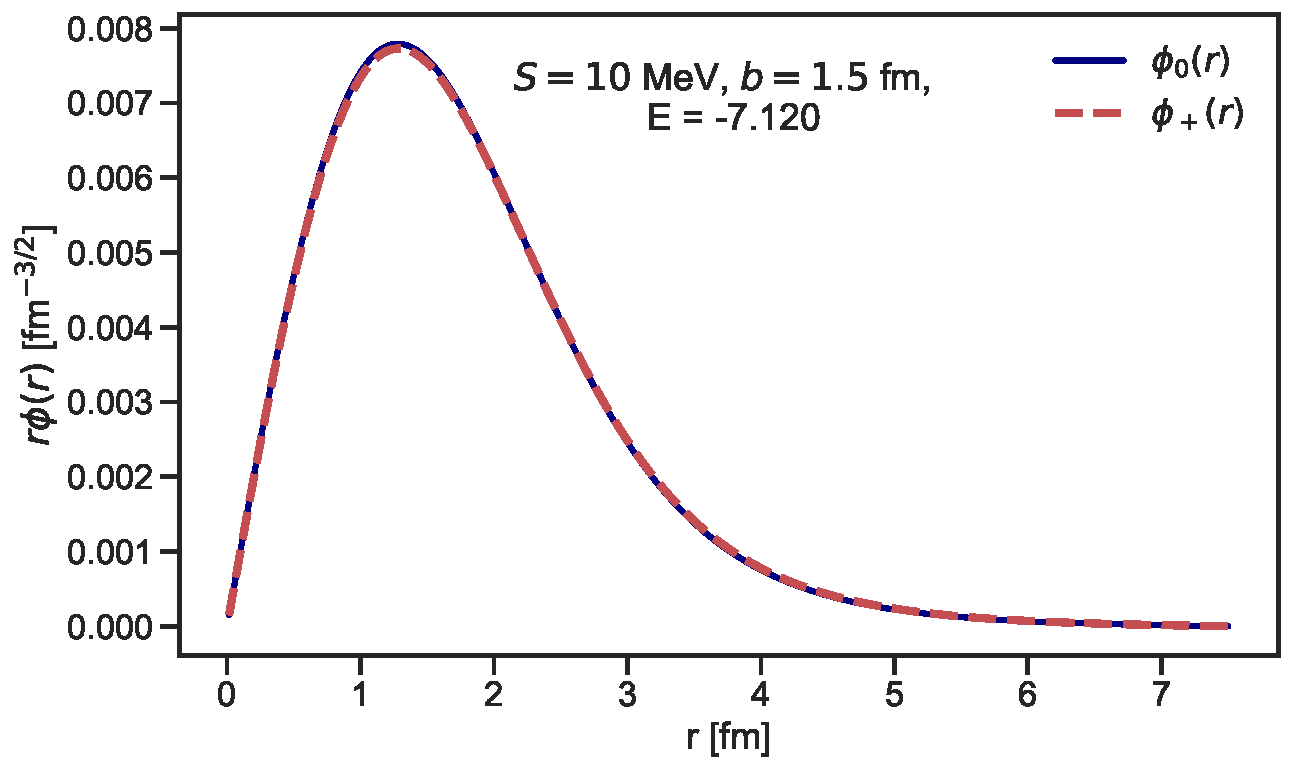
\includegraphics[width=\linewidth]{Figures/Integralplot_CoupledSystem.pdf}
	\end{sidecaption}
\end{figure}
Compared to \ref{fig:integralplot} the difference is negligible even accounting for the mass difference for the pions and nucleons ($m_N, m_P$). This means we can to a good estimation continue using only one pion wave function in our nuclear model. 
\chapter{Angular distribution}\label{sec:Angular}
\begin{figure}[H]
	\begin{sidecaption}{Angular distribution with the parameters $S=86.2$ MeV and $b=3.8$ fm using the relativistic density of states }[fig:Angular1]
		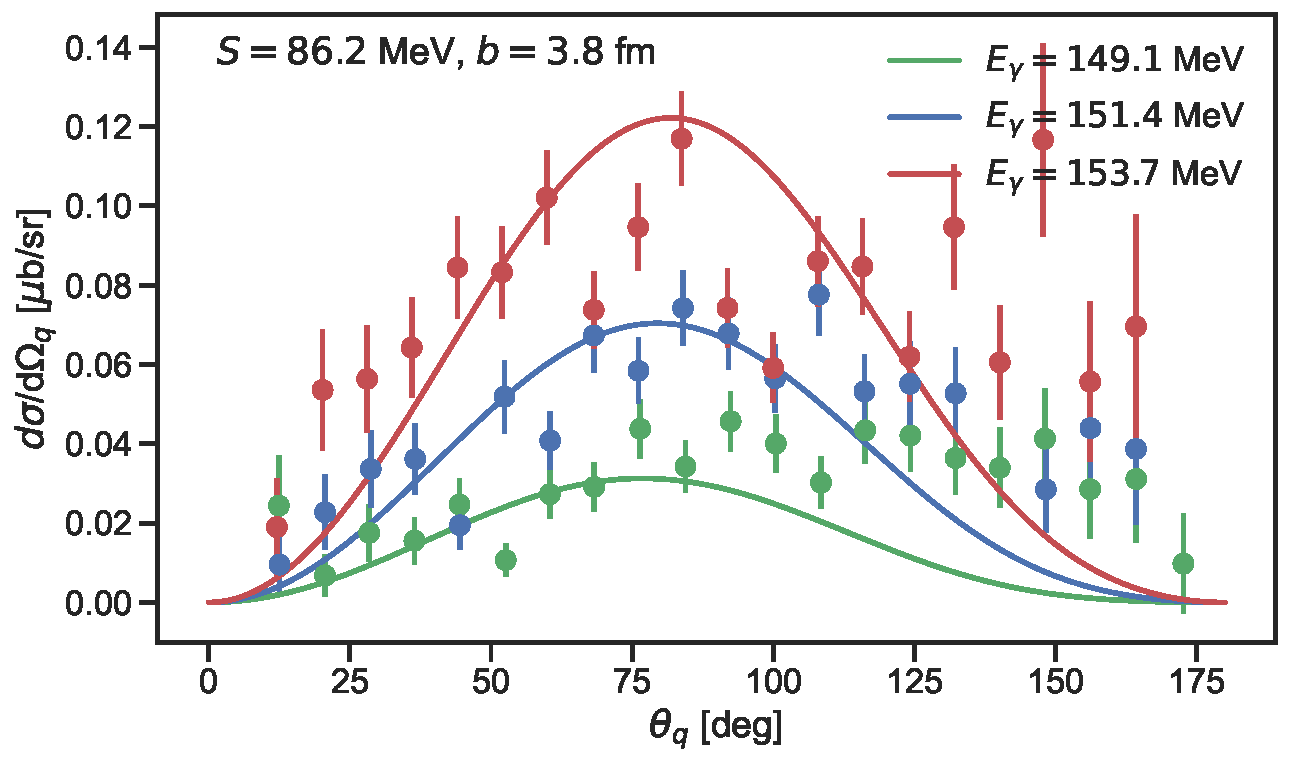
\includegraphics[width=\linewidth]{Figures/MultiDiffcross_rel.pdf}
	\end{sidecaption}
\end{figure}
\begin{figure}[H]
	\begin{sidecaption}{Angular distribution with the parameters $S=45.4$ MeV and $b=3.9$ fm using the relativistic density of state}[fig:Angular1]
		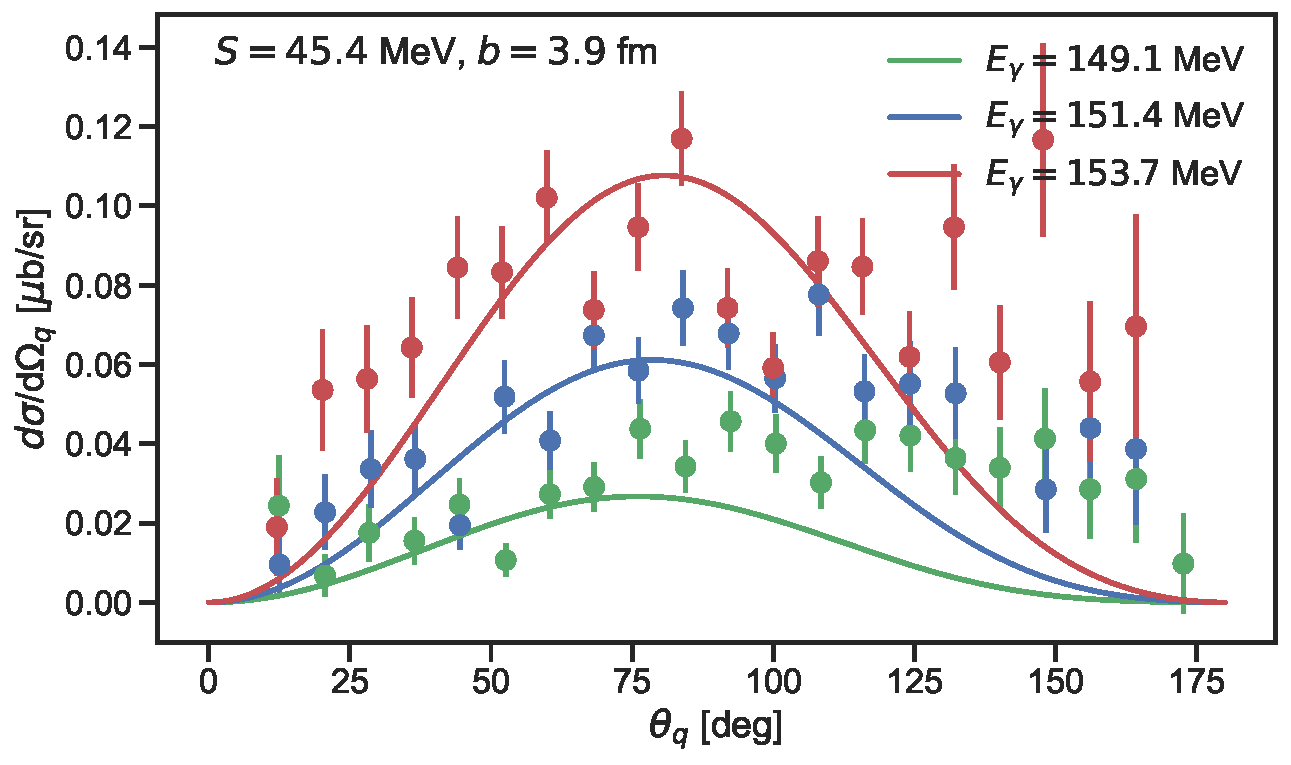
\includegraphics[width=\linewidth]{Figures/MultiDiffcross_rel_2.pdf}
	\end{sidecaption}
\end{figure}
\begin{figure}[H]
	\begin{sidecaption}{Angular distribution with the parameters $S=35$ MeV and $b=4.0$ fm using the relativistic density of state}[fig:Angular3]
		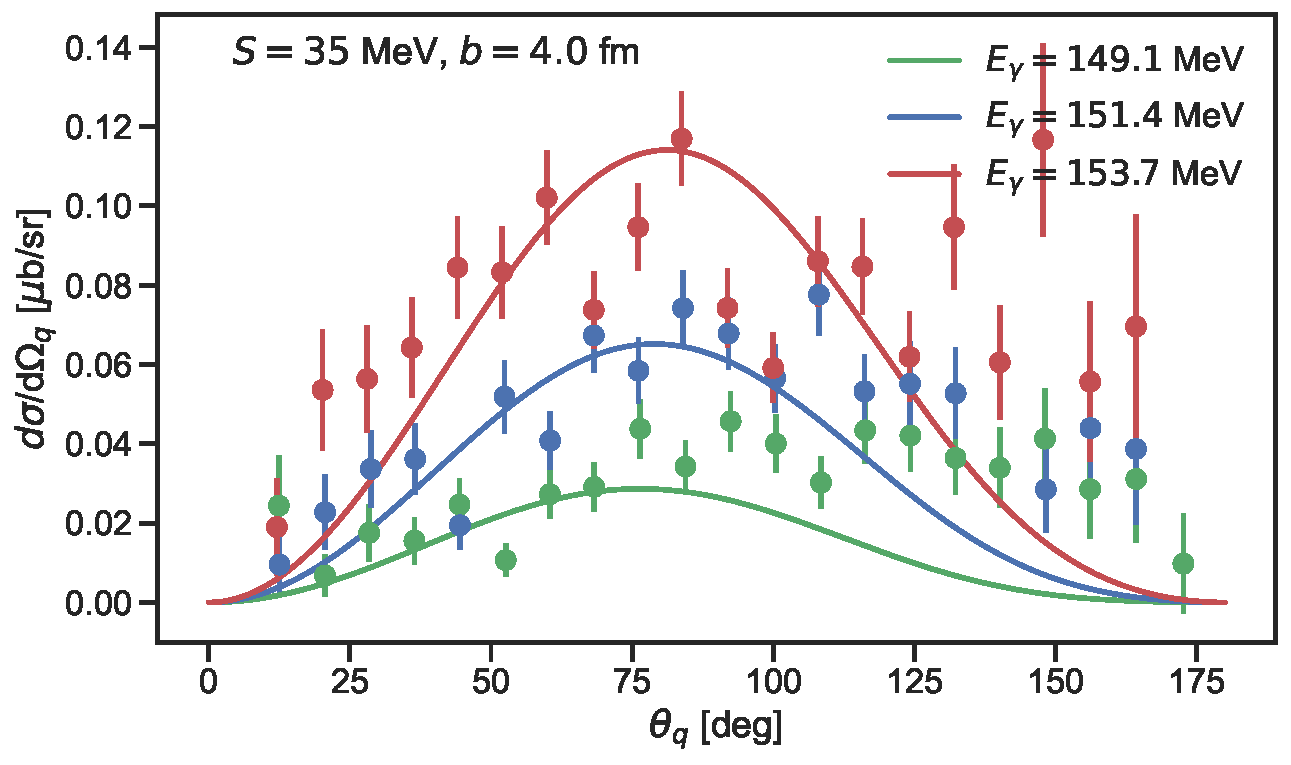
\includegraphics[width=\linewidth]{Figures/MultiDiffcross_rel_3.pdf}
	\end{sidecaption}
\end{figure}


\begin{figure}[H]
	\begin{sidecaption}{Angular distribution with the parameters $S=86.2$ MeV and $b=3.8$ fm using the non-relativistic density of states }[fig:Angular1]
		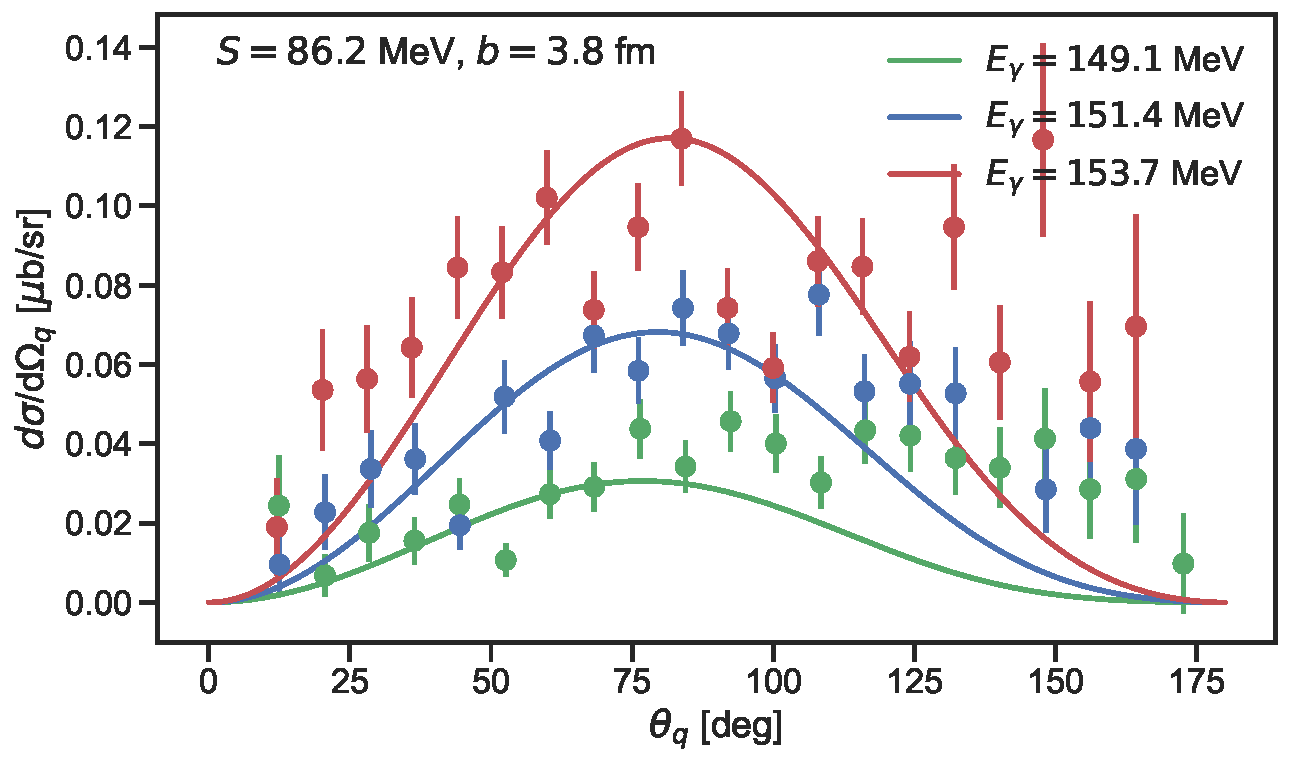
\includegraphics[width=\linewidth]{Figures/MultiDiffcross_nonrel_1.pdf}
	\end{sidecaption}
\end{figure}
\begin{figure}[H]
	\begin{sidecaption}{Angular distribution with the parameters $S=45.4$ MeV and $b=3.9$ fm using the non-relativistic density of state}[fig:Angular1]
		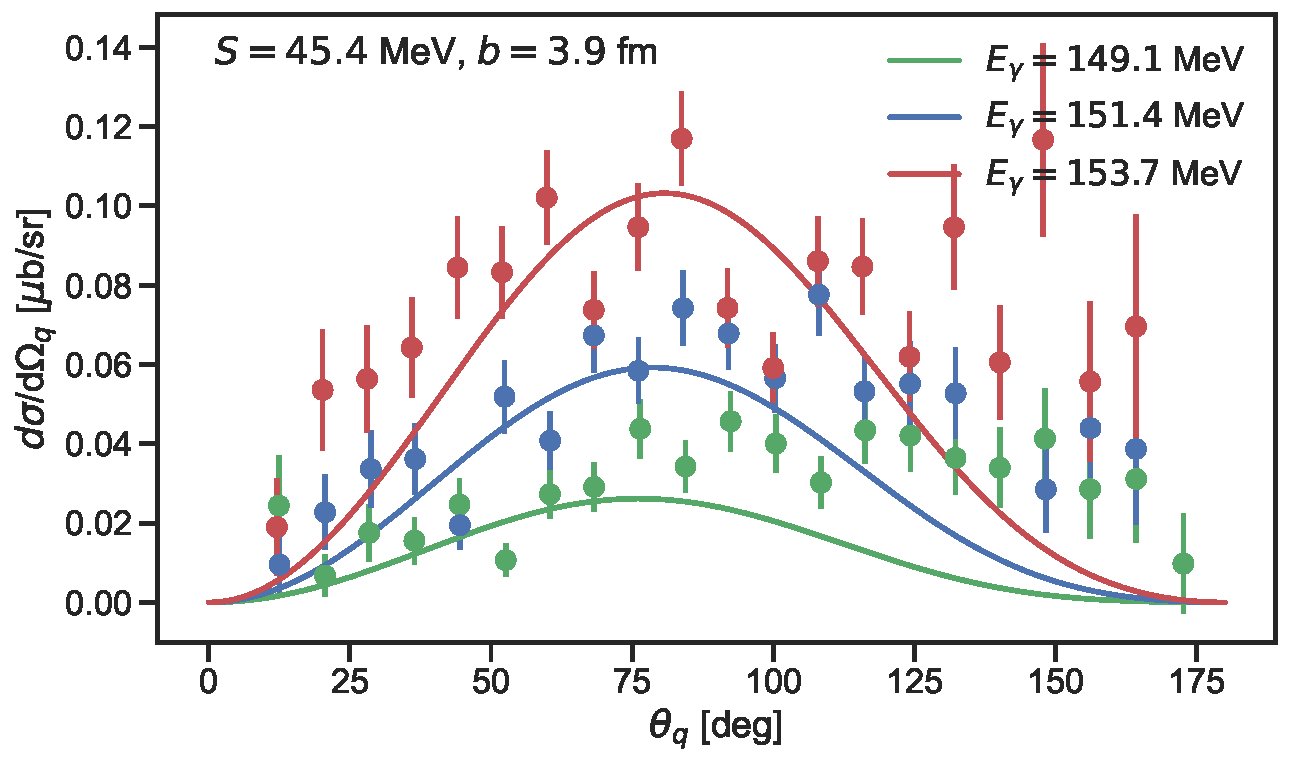
\includegraphics[width=\linewidth]{Figures/MultiDiffcross_nonrel_2.pdf}
	\end{sidecaption}
\end{figure}
\begin{figure}[H]
	\begin{sidecaption}{Angular distribution with the parameters $S=35$ MeV and $b=4.0$ fm using the non-relativistic density of state}[fig:Angular3]
		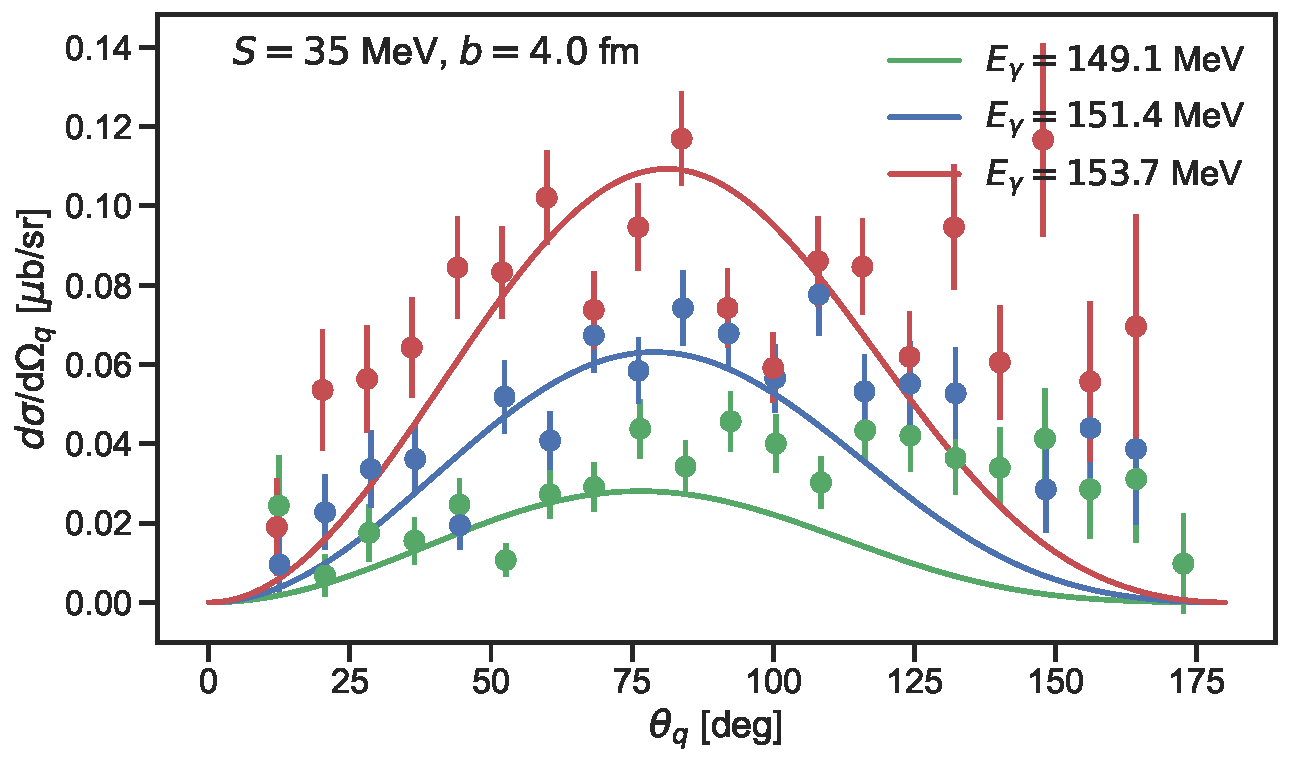
\includegraphics[width=\linewidth]{Figures/MultiDiffcross_nonrel_3.pdf}
	\end{sidecaption}
\end{figure}

